\chapter{Alimentation à découpage Flyback pour chargeur de batterie}

Il s’agit d’utiliser le montage de la figure suivante pour réaliser un chargeur de batterie de tension nominale 24V.

\begin{figure}[h]
\centering
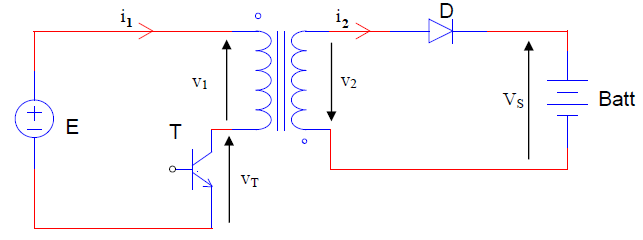
\includegraphics[width=0.8\linewidth]{TD_Flyback/fig/FlybackBatterie.png}
\end{figure}

On note $n_1$ et $n_2$ les nombres de spires respectifs au primaire et au secondaire, le rapport de transformation étant
noté $m$, l'inductance magnétisante primaire sera quant à elle notée $L_1$, la fréquence de découpage $f$, le rapport
cyclique $\alpha$.

La batterie initialement déchargée a une tension à ses bornes $V_{S0} = 20V$. On arrêtera sa charge lorsque la tension
à ses bornes atteindra $V_{S1} = 26 V$. Néanmoins, dans toute l’étude, cette tension batterie, notée $V_S$, sera supposée
constante à l’échelle de temps du découpage.

En débutant la charge de la batterie, on suppose que l'alimentation fonctionne en régime critique avec un rapport cyclique $\alpha_0$, le courant moyen dans la batterie est alors égal à $I_{S0}$.

\vspace{0.25cm}
Valeurs numériques : $E = 300V$ ; $f = 20 kHz$ ; $\alpha_0 = 0.5$ ; $I_{S0} = 10 A$.


\begin{enumerate}

\item \textbf{Début de charge}
\begin{enumerate}
\item Donner l’expression du théorème d’Hopkinson liant $n_1$, $i_1$, $n_2$ et $i_2$ à $R$ réluctance de la ferrite (inverse de l’inductance spécifique $A_L$),  et $\varphi$ flux élémentaire dans celle-ci.
\item Représenter sur une période de découpage l’allure des signaux $i_1$, $i_2$, $\varphi$, $v_T$ et $v_1$.
\item En déduire l'expression de la tension de sortie $V_S$ en fonction de $E$, $m$ et $\alpha_0$. En déduire la valeur numérique de $m$.
\item Déterminer l’expression du courant moyen de sortie noté $I_{S0}$ en fonction de $L_1$, $\alpha_0$, $m$, $E$ et $f$. En
déduire la valeur numérique de l’inductance $L_1$.
\item Calculer de deux façons différentes l’énergie $W_D$ fournie par cycle de découpage à la batterie.
\item Calculer numériquement cette énergie $W_D$ et en déduire le temps de charge à courant constant pour une batterie de `` capacité'' 25 Ah.
\end{enumerate}
\item \textbf{Fin de charge}

Lors de la charge, la tension de sortie évolue lentement de $V_{S0}$ à $V_{S1}$, le rapport cyclique étant maintenu à $\alpha_0$.
\begin{enumerate}
\item Comment le régime de conduction de l’alimentation a-t-il été modifié ?
\item  Représenter sur une période de découpage l’allure des signaux $ i_1$, $i_2$, $v_T$ et $v_1$.
\item Quelle est la durée de conduction de la diode D ?
\item Que vaut maintenant l’énergie transférée par cycle ? En déduire le courant moyen $I_S$ fourni à la batterie.
\item Quelle valeur $\alpha_1$ faudrait-il donner au rapport cyclique pour fournir ensuite un courant moyen de charge de batterie 
$I_{S1} = I_{S0}/10$ ?
\end{enumerate}

\item \textbf{Limite de saturation}

On se place en régime critique (début de charge)

\begin{enumerate}
\item Déterminer l’expression de l'induction maximale dans la ferrite en fonction de E, $\alpha$, T, $n_1$ et $A_e$, surface effective de cette ferrite.
\item En déduire l’expression de la valeur minimale $A_{e\ min}$ de cette ferrite pour empêcher toute saturation du matériau : on notera pour cela $B_{sat}$ la valeur de l’induction au voisinage de la saturation.
\end{enumerate}

\item \textbf{Surface de la fenêtre de bobinage}

On reste en régime critique (début de charge)

\begin{enumerate}
\item En utilisant les résultats de la première partie, déterminer la valeur efficace $I_{1\ eff}$ du courant dans le transistor en fonction du courant de sortie $I_s$, de $m$ et $\alpha$.
\item Faire de même pour exprimer la valeur efficace $I_{2\ eff}$ du courant secondaire en fonction de $I_s$ et $\alpha$.
\item La densité de courant choisie pour ces deux bobinages réalisés en fil de cuivre est $\delta$. Déterminer l'expression de la surface totale de cuivre, notée $S_{T\ Cu}$, en fonction de $I_s$, $\delta$, $n_2$ et $\alpha$. Comparer les surfaces de cuivre primaire et secondaire.
\item En déduire la surface minimale de la fenêtre de bobinage, notée $S_B$, si l’on choisit un coefficient de bobinage $k_B$ ($S_{T\ Cu} = k_B.S_B$).
\end{enumerate}

\item \textbf{Choix du noyau magnétique}

\begin{enumerate}
\item A partir des résultats des questions précédentes, déterminer l'inégalité que doit vérifier le produit $A_e.S_B$ de cette alimentation en fonction de $B_{sat}$, $P_s$, $T$, $k_B$, $\delta$ et $\alpha$.
\item Calculer cette valeur minimale en $mm^4$ pour les valeurs numériques suivantes :

\begin{center}
$P_s = 200 W$ ; $\alpha = 0.5$ ; $k_B = 0.5$ ; $B_{sat} = 0.4 T$ ; $\delta = 5 A.mm^{-2}$ ; $f = 20 kHz$.
\end{center}

\newpage
\item Choisir un noyau parmi la liste suivante pour laquelle on donne les valeurs de $A_e$, $S_B$ et $A_L$ fournies par le constructeur (on rappelle que $A_L$ désigne l’inductance spécifique pour une spire), tous ces noyaux étant réalisés avec le même matériau $N41$.

\vspace{1mm}
\begin{tabular}{| c | c | c | c | c |}
	\hline
	\multirow{2}*{Noyau} & \multirow{2}*{$A_e\ (mm^2)$} & \multirow{2}*{$S_B \ (mm^2)$} & $A_L$ sans entrefer & $A_L$ entrefer 0.5 mm\\
	 & & & (nH) & (nH)\\
	\hline
	%RM4 & 11 & 14 & 63 & - - - \\
	\hline
	RM6 & 31 & 32 & 3100 & - - -\\
	\hline
	RM8 & 55 & 57 & 4100 & 160\\
	\hline
	RM10 & 90 & 93 & 5500 & 250\\
	\hline
	RM12 & 125 & 128 & 6000  & 300 \\
	\hline
	RM14 & 170 & 176 & 6800 & 400 \\
	\hline
\end{tabular}

\vspace{1mm}

\item Pour ce choix de noyau, déterminer alors les nombres de spires minimaux $n_1$ et $n_2$ pour limiter l’induction maximale dans la ferrite à $B_{sat}$. Pour ces calculs, on choisira  ``au mieux'' ces valeurs de nombres de spires pour les valeurs numériques ci-dessus.

\item Un entrefer sera-t-il nécessaire afin d’obtenir l’inductance $L_1$ souhaitée ?

\end{enumerate}

\begin{figure}[h]
\centering
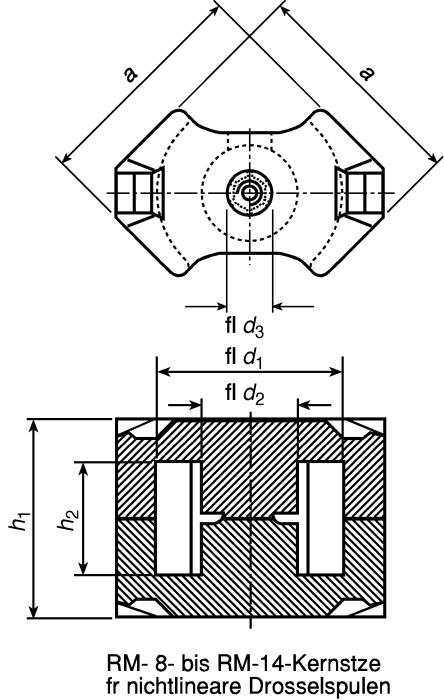
\includegraphics[width=0.5\linewidth]{TD_Flyback/fig/noyau.png}
\end{figure}

\end{enumerate}